% Titolo della sezione e label. Vi consiglio, per questioni di ordine mentale e rapidità successiva di reference, di etichettare le label in modo sensato, con riferimento chiaro a cosa si sta etichettando. Quindi sec:nomesezione per una sezione, im:nomeimmagine per una immagine, e via dicendo.
\section{Introduction}\label{sec:introduction} 
The Project 5 is a real application of the techniques of EEG signal processing studied in class on a real case. 
\subsection{Description of the case}\label{subsec:desc}
The case is the 2019 Cybathlon race, where a pilot have to interact with a game using a BMI, the pilot use 2 motor imagery to control the game interface. The motor imagery is both hands and both feet. In a period of 3 month the pilot in 11 sessions performed two kinds of runs. Offline where the pilot not have real feedback, used only for calibration, and Online session where pilot receive visual stimulus as a feedback of his commands. The pilot on the online runs can see on the screen two colored bars related to the imagery tasks. The colored bars is filled according with the output of the classifier on actual signals.
\subsection{Data Description}\label{subsec:datadesc}
The 11 sessions are composed with some gdf file, containing all information regarding the run type and ordered by timestamp:
\begin{itemize}
    \item \textbf{$20190502_F1$} Executed in 02nd of May 2019 and composed by 3 offline runs and 3 online runs.
    \item \textbf{$20190506_F1$} Executed in 05th of May 2019 and composed by 1 long offline runs and 5 online runs.
    \item \textbf{$20190513_F1$} Executed in 13th of May 2019 and composed by 1 long offline runs and 3 online runs.
    \item \textbf{$20190521_F1$} Executed in 21th of May 2019 and it started with an online run, followed by 3 offline runs and closed with a last online run.
    \item \textbf{$20190610_F1$} Executed in 06th June 2019 and composed only by an online run. 
    \item \textbf{$20190624_F1$} Executed in 24th June 2019 and composed only by an online run. 
    \item \textbf{$20190627_F1$} Executed in 27th June 2019 and composed only by an online run. 
    \item \textbf{$20190701_F1$} Executed in 1st July 2019 and composed by 7 online runs. 
    \item \textbf{$20190709_F1$} Executed in 9th July 2019 and started with 2 online runs followed by 4 offline runs anc closed with a last online run. 
    \item \textbf{$20190711_F1$} Executed in 11th July 2019 and composed by 2 online runs. 
    \item \textbf{$20190715_F1$} Executed in 15th July 2019 and composed by 2 online runs. 
\end{itemize}
\newpage
\subsection{Pipeline description}\label{subsec:pipeline}
For this project the first important thing to do is configure the project with fundamental parameter used for all tasks, after that we can proceed loading data session keeping divided for each session online data from offline data. The main idea is to analyze offline sessions before computing fisher score and extracting channel and frequencies that could be used as discriminant for the classifier, create a classifier for each session, test classifiers with online runs measuring the performance. On Figure 1 we can see the 4 main component that compose the pipeline. I used factory/builder pattern to approach the problem, During the first phase we have to process data in order to identify a good discriminant for feature selection, during this phase we'll use only the first part of the pipeline for analyze offline sessions. Only in the second phase after feature selection will use the complete pipeline. 
\begin{figure}[h]
    \centering
    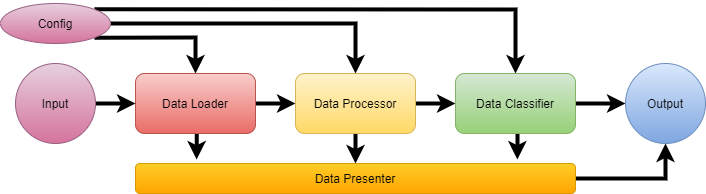
\includegraphics[width=0.8\textwidth]{Figure/NR_Pipeline.png}
    \caption{Pipeline description.}
    \label{fig:Pipeline}
\end{figure}\\
\begin{itemize}
    \item Data Loader: Responsible of data loading and early processing. This component is a standalone class with collection container for the data in the gdf files. Another important responsibility of this class is the early data processing with spatial filtering and spectrogram computing.
    \item Data Processor: The class responsible for the data processing and manipulation during analysis procedure. This class do all step necessary to extract the information necessary for the feature selection and classifier training. 
    \item Data Classifier: This is the last component of the pipeline, another class with all method necessary for the dataset (trainset and testset) and classifier train test operation.
    \item Data Presenter: The only class of the pipeline parallel to all component with only static methods. Each component of the pipeline have a reference to this class, in order to call necessary method to plot output and chart. This component of the pipeline not have class member except the output configuration.
\end{itemize}
The pipeline was created for allow to each module easy access to output of previous module. Data processor has a reference of data loader class for get data, and data classifier have a reference to data processor. With this method each component can easily access to the past history of the data.

